%Version 3.1 December 2024
% See section 11 of the User Manual for version history
%
%%%%%%%%%%%%%%%%%%%%%%%%%%%%%%%%%%%%%%%%%%%%%%%%%%%%%%%%%%%%%%%%%%%%%%
%%                                                                 %%
%% Please do not use \input{...} to include other tex files.       %%
%% Submit your LaTeX manuscript as one .tex document.              %%
%%                                                                 %%
%% All additional figures and files should be attached             %%
%% separately and not embedded in the \TeX\ document itself.       %%
%%                                                                 %%
%%%%%%%%%%%%%%%%%%%%%%%%%%%%%%%%%%%%%%%%%%%%%%%%%%%%%%%%%%%%%%%%%%%%%

%%\documentclass[referee,sn-basic]{sn-jnl}% referee option is meant for double line spacing

%%=======================================================%%
%% to print line numbers in the margin use lineno option %%
%%=======================================================%%

%%\documentclass[lineno,pdflatex,sn-basic]{sn-jnl}% Basic Springer Nature Reference Style/Chemistry Reference Style

%%=========================================================================================%%
%% the documentclass is set to pdflatex as default. You can delete it if not appropriate.  %%
%%=========================================================================================%%

%%\documentclass[sn-basic]{sn-jnl}% Basic Springer Nature Reference Style/Chemistry Reference Style

%%Note: the following reference styles support Namedate and Numbered referencing. By default the style follows the most common style. To switch between the options you can add or remove “Numbered” in the optional parenthesis.
%%The option is available for: sn-basic.bst, sn-chicago.bst%

%%\documentclass[pdflatex,sn-nature]{sn-jnl}% Style for submissions to Nature Portfolio journals
%%\documentclass[pdflatex,sn-basic]{sn-jnl}% Basic Springer Nature Reference Style/Chemistry Reference Style
\documentclass[pdflatex,sn-mathphys-num]{sn-jnl}% Math and Physical Sciences Numbered Reference Style
%%\documentclass[pdflatex,sn-mathphys-ay]{sn-jnl}% Math and Physical Sciences Author Year Reference Style
%%\documentclass[pdflatex,sn-aps]{sn-jnl}% American Physical Society (APS) Reference Style
%%\documentclass[pdflatex,sn-vancouver-num]{sn-jnl}% Vancouver Numbered Reference Style
%%\documentclass[pdflatex,sn-vancouver-ay]{sn-jnl}% Vancouver Author Year Reference Style
%%\documentclass[pdflatex,sn-apa]{sn-jnl}% APA Reference Style
%%\documentclass[pdflatex,sn-chicago]{sn-jnl}% Chicago-based Humanities Reference Style

%%%% Standard Packages
%%<additional latex packages if required can be included here>

\usepackage{graphicx}%
\usepackage{multirow}%
\usepackage{amsmath,amssymb,amsfonts}%
\usepackage{amsthm}%
\usepackage{mathrsfs}%
\usepackage[title]{appendix}%
\usepackage{xcolor}%
\usepackage{textcomp}%
\usepackage{manyfoot}%
\usepackage{booktabs}%
%\usepackage{algorithm}%  % Not used in this paper
%\usepackage{algorithmicx}%  % Not used in this paper
%\usepackage{algpseudocode}%  % Not used in this paper
\usepackage{listings}%
\usepackage{subfig}%
\usepackage{tikz}
\usepackage{nicefrac}

\usepackage{pgf}
\usepackage{lmodern}
\usepackage{import}

\usepackage{amsmath, amssymb}
%\usepackage{siunitx}        % Not used in this paper
\usepackage{natbib}
\usepackage{multirow}
\usepackage{comment}
%\usepackage{mathptmx}
%%%%

%%%%%=============================================================================%%%%
%%%%  Remarks: This template is provided to aid authors with the preparation
%%%%  of original research articles intended for submission to journals published
%%%%  by Springer Nature. The guidance has been prepared in partnership with
%%%%  production teams to conform to Springer Nature technical requirements.
%%%%  Editorial and presentation requirements differ among journal portfolios and
%%%%  research disciplines. You may find sections in this template are irrelevant
%%%%  to your work and are empowered to omit any such section if allowed by the
%%%%  journal you intend to submit to. The submission guidelines and policies
%%%%  of the journal take precedence. A detailed User Manual is available in the
%%%%  template package for technical guidance.
%%%%%=============================================================================%%%%

%% as per the requirement new theorem styles can be included as shown below
\theoremstyle{thmstyleone}%
\newtheorem{theorem}{Theorem}%  meant for continuous numbers
%%\newtheorem{theorem}{Theorem}[section]% meant for sectionwise numbers
%% optional argument [theorem] produces theorem numbering sequence instead of independent numbers for Proposition
\newtheorem{proposition}[theorem]{Proposition}%
%%\newtheorem{proposition}{Proposition}% to get separate numbers for theorem and proposition etc.

\theoremstyle{thmstyletwo}%
\newtheorem{example}{Example}%
\newtheorem{remark}{Remark}%

\theoremstyle{thmstylethree}%
\newtheorem{definition}{Definition}%

\setlength{\parskip}{1em}   % space between paragraphs
\setlength{\parindent}{1.5em} % optional: no indentation
\raggedbottom
%%\unnumbered% uncomment this for unnumbered level heads

\begin{document}

\title[Article Title]{Using Peridynamics to Model Hydrogen Embrittlement in Stainless Steel}

%%=============================================================%%
%% GivenName	-> \fnm{Joergen W.}
%% Particle	-> \spfx{van der} -> surname prefix
%% FamilyName	-> \sur{Ploeg}
%% Suffix	-> \sfx{IV}
%% \author*[1,2]{\fnm{Joergen W.} \spfx{van der} \sur{Ploeg}
%%  \sfx{IV}}\email{iauthor@gmail.com}
%%=============================================================%%

\author{\fnm{Maddie A.} \sur{Schmitz}}\email{madison.schmitz@austin.utexas.edu}
\author{\fnm{John T.} \sur{Foster}}\email{john.foster@utexas.edu}

\affil{\orgdiv{The Oden Institute for Computational Engineering and Sciences},
           \orgname{The University of Texas at Austin},
           \orgaddress{\city{Austin}, \postcode{78712}, \state{TX}, \country{USA}}}

\abstract{Abstract}


\keywords{Keywords}

%%\pacs[JEL Classification]{D8, H51}

%%\pacs[MSC Classification]{35A01, 65L10, 65L12, 65L20, 65L70}

\maketitle

\section{Introduction}\label{sec1}
%%%%%%%%%% Figure
\begin{figure}[!b]
\centering
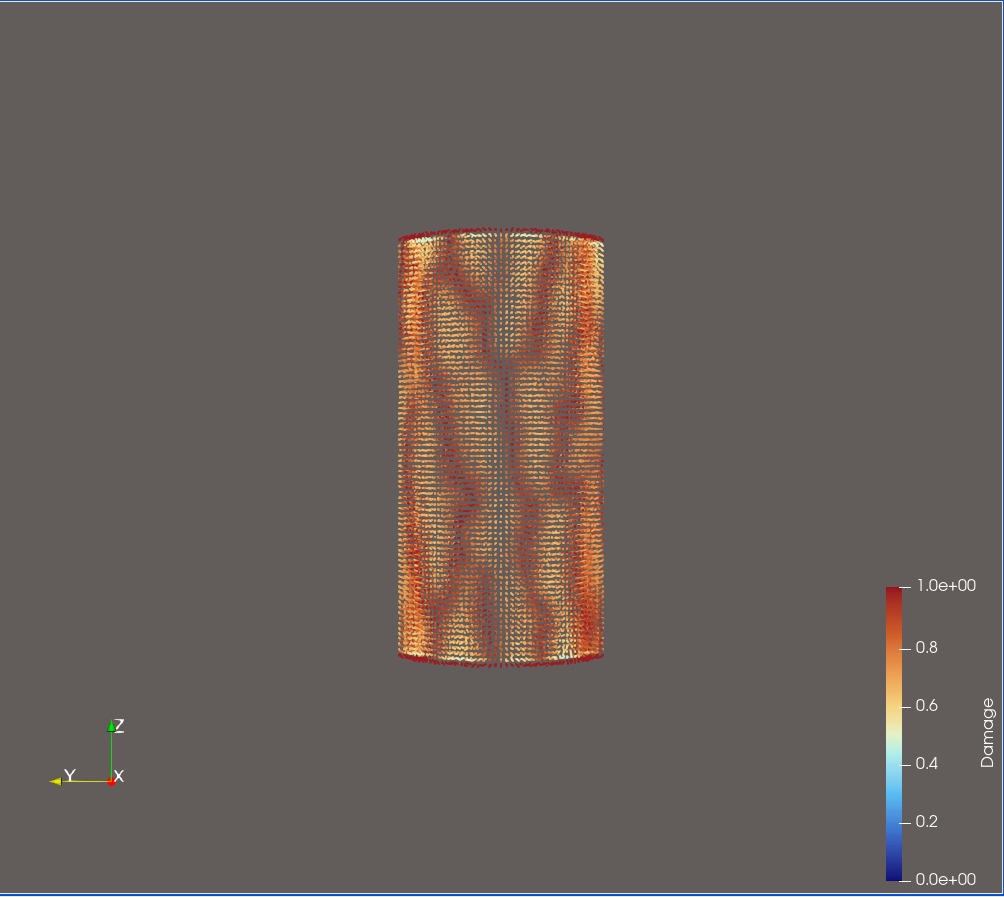
\includegraphics[width=\linewidth]{figs_HE/HE_0_frame_1150.jpg}
\caption{Optimized nodal thickness distributions for the 1D bar obtained by minimizing strain energy density (green) and the $L^1$ norm of damage (red). The damage-optimized profile achieves fracture suppression with substantially less added material than the strain energy density-optimized profile.}
\label{fig:optThickDamageStrainEnergyDenOverlayed}
\end{figure}

\section{Methods - The Peridynamic Formulation}\label{sec2}

\subsection{Methods - Subsection}



%%%%%%%%%%%%%%%%%%%%%%%%%%
\section{Results}\label{sec5}
\subsection{Results - Subsection 1}\label{subsec5a}

\subsection{Limitations}
Limitations

\section{Conclusion}\label{sec7}
Conclusions


\section{Supplementary information}\label{sec8}

\bmhead{Acknowledgements}\label{sec9}

\section*{Declarations}\label{sec10}

\begin{itemize}
\item \textbf{Funding:} Not applicable.
\item \textbf{Conflict of interest:} The authors declare no conflict of interest.
\item \textbf{Ethics approval:} Not applicable.
\item \textbf{Consent for publication:} Not applicable.
\item \textbf{Data availability:} The datasets generated during this study are available from the corresponding author on reasonable request.
\item \textbf{Code availability:} 
\item \textbf{Author contributions:} 
\end{itemize}

%%===========================================================================================%%
%% If you are submitting to one of the Nature Portfolio journals, using the eJP submission   %%
%% system, please include the references within the manuscript file itself. You may do this  %%
%% by copying the reference list from your .bbl file, paste it into the main manuscript .tex %%
%% file, and delete the associated \verb+\bibliography+ commands.                            %%
%%===========================================================================================%%

\bibliography{references_PD_paper}\label{sec11}
%% if required, the content of .bbl file can be included here once bbl is generated
%%\input sn-article.bbl

\end{document}
